\section{Data Transmission Packet Processing Module}

To transmit data packets from the event bus, the network stack must
acquire the variable length packets, place them into larger udp
datagrams, set the metadata fields, and transmit them. However, we
must also save a copy of each packet (for possible retransmission),
and respond to a retransmission request should one occur during the
normal stream of data transmission.

To enable retransmission we have a packet TX FIFO with space for 256
1024-byte packets; a data packet should never exceed 600 bytes. This
FIFO also gives us headroom should the TX Fifo fill due to
insufficient access to the TX Mux interface. Note that, on average, we
have more than enough TX bandwidth -- but in the short run it is
possible to fill the TX fifo and thus need to buffer packets in the
in-memory FIFO.

This interface is heavily pipelined, as data bus packet transmission
is not viewed as an event-critical process.

We have various FIFOs and synchronization interfaces to guarantee our
goal of, within an ECYCLE, being able to service:

\begin{itemize}
\item The arrival of two new data bus packets and their subsequent
  memory writes to the fifo.
\item The placement of two packets in the memory fifo into the output
  FIFO for transmission
\item The retrieval of one packet for retransmission
\end{itemize}

 \begin{figure}
\begin{centering}
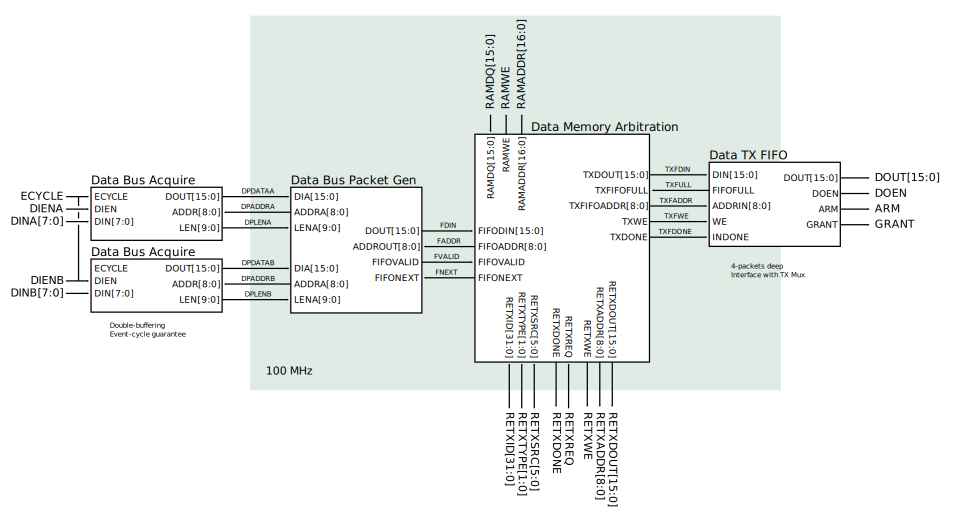
\includegraphics[scale=0.7]{data.svg}
\end{centering}
\caption{Data Transmission Interface}
\label{data}
\end{figure}


\subsection{Data Bus Acquire}
The data bus acquire interface takes a data bus packet and: 

1. event-cycle aligns it, so it is guaranteed to be available on the
   next ecycle.
2. converts it to a 16-bit-wide packet
3. measures the length

\subsubsection{Interface and Implementation} 
 \begin{figure}
\begin{centering}
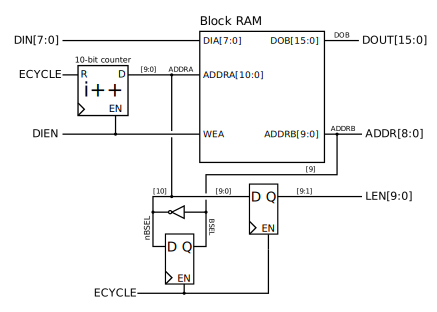
\includegraphics[scale=0.8]{data.acquire.svg}
\end{centering}
\caption{Data Bus Acquire.}
\label{data.acquire}
\end{figure}

It uses a double-buffer approach. On the cycle following
\signal{ECYCLE}-assertion, \signal{LEN[9:0]} contains the length of
the packet in words, not bytes; if \signal{LEN[9:0]} =0 then there is
no packet awaiting transmission.

\signal{BSEL} selects which buffer. \signal{ADDR[8:0]} selects the
output word.

\subsection{Data Bus Packet Gen}
The data bus packet generator generates one or two datagrams every
event cycle, which are ready for processing at the end of the event
cycle.
The data bus packet generator also assigns the 32-bit sequence ID to
each packet based upon packet source and type.


\subsubsection{Interface}
\begin{figure}
\begin{centering}
\includegraphics[scale=0.8]{data.packetgen.svg}
\end{centering}
\caption{Data Bus Transmission packet generation.}
\label{data.packetgen}
\end{figure}

\begin{figure}
\begin{centering}
\includegraphics[scale=0.8]{data.packetgen.fsm.svg}
\end{centering}
\caption{Data Bus Transmission packet generation finite state machine.}
\label{data.packetgen.fsm}
\end{figure}

The input interface interoperates with the Data Bus Acquire module.
Output packets are simply written to the downstaream FIFO. 



\subsubsection{implementation}
To store a packet, we examine both \signal{LENA[9:0]} and
\signal{LENB[9:0]} to check for non-zero values each Event Cycle.
Should a packet have a non-zero value, we begin copying it into the
output FIFO. Througout the transmission of this packet, we lock on to
the packet source and type, and use this to look up the current value
of sequence number via \signal{SEQDO[31:0]} .

Then, we use the UDPheader to write the relevant packet header data.
\signal{TLEN } is two greater than the input \signal{LEN[9:0]} to
account for the addition of the sequence ID in the header. The
destination port is calculated from the latched \signal{SRC[5:0]} and
\signal{TYP[1:0]}.

Finally, the sequence ID is written to the fifo and the packet is
committed by incrementingthe input fifo pointer, \signal{FADDR[10:9]}.

The fifo output stage, running at 100 MHz, simply checks if the input
fifo pointer (registered as \signal{FIFONUM}) is different from the
output fifo pointer and asserts \signal{FIFOVALID} if so.

\subsection{Data Output FIFO}
The data output fifo is the fifo that buffers data packets to be
transmitted to deal with the fact that while our Data TX hit rate is
only 64 packets out of every 100 slots (1 ms) we could have them all
bunch up, and that would be, in the words of T-Rex ``most
unfortunate''.

The fifo is constrained to -always- take input from the packet
generator, and presents a series of 1k-deep packet interfaces.




\begin{figure}
\begin{centering}
\includegraphics[scale=0.8]{data.outputfifo.svg}
\end{centering}
\caption{Data Bus Transmission output FIFO.}
\label{data.outputfifo}
\end{figure}

\subsection{Retransmission Buffer Rate Limiter}
This module extracts out the relevant packet metadata and writes it to
the retransmission buffer, performing the necessary clock-rate
conversion in the process. It has an internal 8-packet buffer to
smooth out the requests for buffer writing, since the ReTX Buffer
could be in the middle of a packet.


